\documentclass{article}
\usepackage[utf8]{inputenc}
\usepackage[spanish]{babel}
\usepackage{amsmath}
\usepackage{amssymb}
\usepackage{booktabs}
\usepackage{longtable}
\usepackage{geometry}
\usepackage{graphicx}
\usepackage{float}

\geometry{a4paper, margin=1in}

\begin{document}

\begin{titlepage}
		
		\begin{center}
			
			{\Large { Maestría en Ciencia de Datos e Inteligencia Artificial} }\\[1cm]
			
\includegraphics[scale=0.15]{logo.png}
			\\[1cm]
			{\Huge \textsc{Tarea 02}}\\[0.7cm]
			{\Huge Applied high performance computing}\\[1cm]
			{\Large Informe Comparativo de Escalabilidad de Random Forest\\en Particiones SLURM: Debug vs Standard}\\[2cm]
			
			\begin{minipage}[l]{0.4\textwidth}
				\begin{flushleft}
					\textbf{\textsf{Profesor:}}\\
					\large Jose Antonio Fiestas Iquira\\ 
					\linespread{4}
					\large .\\ 
				\end{flushleft}
			\end{minipage}
			\begin{minipage}[l]{0.4\textwidth}
				
				\begin{flushright}
					\textbf{\textsf{Integrantes:}}\\
					\linespread{1}
					\large Morocho Caballero, Rodolfo\\
					\large Ramirez Martel, Max Houston\\
                    \large Velasquez Santos, Alberto Valentin\\
				\end{flushright}
                \date{\today}
			\end{minipage}
			
		\end{center}
        \end{titlepage}
\newpage                
        
\begin{abstract}
Este informe presenta un análisis de rendimiento y escalabilidad de un clasificador Random Forest
(Bosque Aleatorio) implementado con scikit-learn sobre un conjunto de datos sintéticos, variando el
número de hilos de procesamiento ($P$) y el tamaño de la muestra ($N$). Los resultados demuestran una
aceleración significativa en el tiempo de ajuste ($T_{fit}$) con el aumento de $P$, aunque con una eficiencia
que disminuye progresivamente debido a la sobrecarga paralela. También se observa que el tiempo de
ajuste escala de forma super-lineal con el tamaño de la muestra, lo cual es consistente con la complejidad
algorítmica esperada. La exactitud del modelo se mantuvo alta y estable en todas las ejecuciones.
\end{abstract}

\section{Introducción}
Este informe analiza el rendimiento del entrenamiento de un clasificador \textbf{Random Forest} en función del número de hilos de procesamiento ($P$) y el tamaño de la muestra ($N$), comparando los resultados obtenidos en las particiones de \textbf{SLURM} \texttt{debug} y \texttt{standard}.

\section{Configuración del Experimento}
El experimento se ejecutó sobre una plataforma de Cómputo de Alto Rendimiento (HPC), utilizando el
sistema de colas SLURM (script \texttt{rf.sh}). Se realizaron pruebas variando dos parámetros clave:

\begin{itemize}
    \item \textbf{Número de Hilos} ($P$ o \texttt{n\_jobs}): $P \in \{1, 2, 4, 8, 16, 32\}$
    \item \textbf{Tamaño de la Muestra} ($N$ o \texttt{n\_samples}): $N \in \{100\text{k}, 200\text{k}, 400\text{k}, 800\text{k}\}$
\end{itemize}

Todos los demás hiperparámetros del Random Forest se mantuvieron fijos: \texttt{n\_estimators} = 400, \texttt{max\_depth}
= 20, \texttt{n\_features} = 40. Los tiempos reportados son el promedio de \texttt{reps} = 3 ejecuciones.

\section{Análisis de Resultados entre Particiones}

\subsection{Comparativa de Tiempos de Entrenamiento y Particiones}
La Tabla \ref{tab:tiempos} compara los tiempos de entrenamiento promedio (\texttt{fit\_time\_s\_avg}) entre las particiones \texttt{debug} y \texttt{standard}.

\begin{longtable}{cc|cc|c}
\caption{Tiempos Promedio de Entrenamiento (fit\_time\_s\_avg) en segundos} \label{tab:tiempos} \\
\toprule
\textbf{$N$ (n\_samples)} & \textbf{$P$ (n\_jobs)} & \textbf{Debug (s)} & \textbf{Standard (s)} & \textbf{Diferencia Absoluta (s)} \\
\midrule
\endfirsthead
\multicolumn{5}{c}%
{\tablename\ \thetable: Tiempos Promedio de Entrenamiento (fit\_time\_s\_avg) en segundos (Continuación)} \\
\toprule
\textbf{$N$ (n\_samples)} & \textbf{$P$ (n\_jobs)} & \textbf{Debug (s)} & \textbf{Standard (s)} & \textbf{Diferencia Absoluta (s)} \\
\midrule
\endhead
\bottomrule
\endfoot
\endlastfoot
$100\,000$ & 1 & 274.3691 & 273.3223 & 1.0468 \\
$100\,000$ & 2 & 148.8030 & 141.1416 & 7.6614 \\
$100\,000$ & 4 & 76.5603 & 76.4074 & 0.1529 \\
$100\,000$ & 8 & 42.2916 & 42.7293 & -0.4377 \\
$100\,000$ & 16 & 24.6369 & 24.1222 & 0.5147 \\
$100\,000$ & 32 & 18.8874 & 17.8188 & 1.0686 \\
\midrule
$200\,000$ & 1 & --- & 597.3964 & \texttt{N/A} \\
$200\,000$ & 2 & 326.5193 & 310.9889 & 15.5304 \\
$200\,000$ & 4 & 170.8021 & 167.2803 & 3.5218 \\
$200\,000$ & 8 & 94.0955 & 91.0158 & 3.0797 \\
$200\,000$ & 16 & 54.5251 & 53.9700 & 0.5551 \\
$200\,000$ & 32 & 40.5150 & 39.0745 & 1.4405 \\
\midrule
$400\,000$ & 4 & 373.6588 & 364.0706 & 9.5882 \\
$400\,000$ & 8 & 207.6706 & 212.3651 & -4.6945 \\
$400\,000$ & 16 & 124.0623 & 122.0659 & 1.9964 \\
$400\,000$ & 32 & 90.2325 & 86.4191 & 3.8134 \\
\midrule
$800\,000$ & 8 & 478.4954 & 492.0175 & -13.5221 \\
$800\,000$ & 16 & 284.5556 & 281.8692 & 2.6864 \\
$800\,000$ & 32 & 194.1013 & 194.2279 & -0.1266 \\
\end{longtable}

\paragraph{Observaciones de Particiones:}
El rendimiento de cómputo es \textbf{similar} entre \texttt{debug} y \texttt{standard} (con \texttt{standard} siendo marginalmente más rápida en la mayoría de los casos). Esto implica que las ventajas de cada partición son de naturaleza administrativa (cola, límites de tiempo), no de rendimiento bruto del hardware.

\section{Análisis de Escalabilidad por Hilos ($P$)}

\subsection{Figura 1: Tiempo de Ajuste vs. Número de Hilos}

La Figura \ref{fig:tiempo_ajuste} muestra la reducción del tiempo de entrenamiento al aumentar el número de hilos $P$ (escala logarítmica en el eje Y), lo que confirma que el algoritmo Random Forest es altamente paralelizable.

\begin{figure}[H]
    \centering
    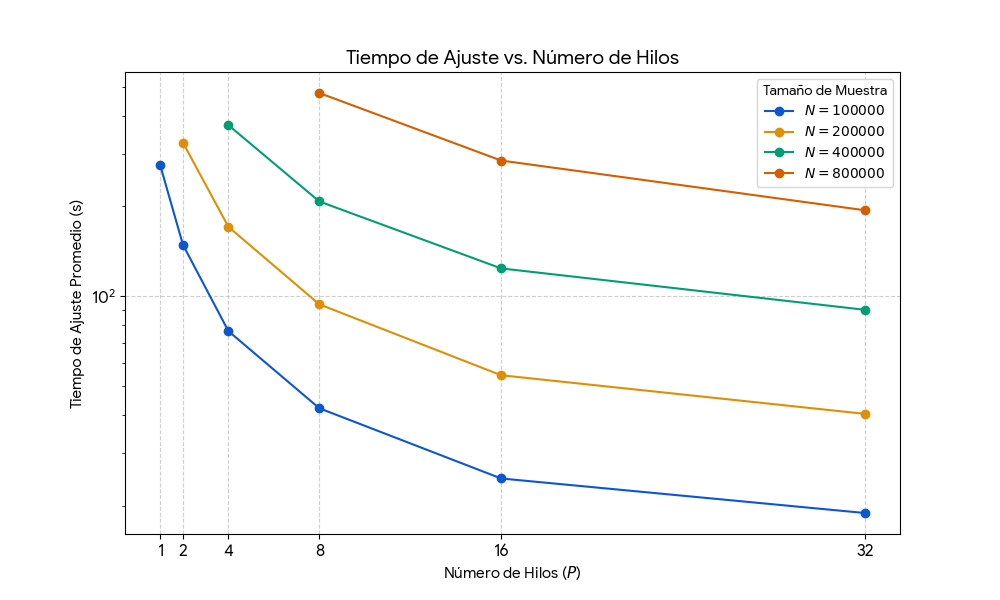
\includegraphics[width=0.8\textwidth]{fit_time_vs_n_samples_p32.png}
    \caption{Figura 1: Tiempo de Ajuste Promedio vs. Número de Hilos ($P$).}
    \label{fig:tiempo_ajuste}
\end{figure}

\paragraph{Conclusiones de la Figura 1 (Tiempo Absoluto):}
\begin{enumerate}
    \item \textbf{Ley de Amdahl Evidente:} Se observa una fuerte disminución de tiempo inicialmente (de $P=1$ a $P=8$). La reducción se hace \textbf{menos pronunciada} de $P=16$ a $P=32$, especialmente para los problemas más grandes ($N=400\,000$ y $N=800\,000$), lo que indica que el \textbf{overhead} y la parte secuencial del código (\textbf{Ley de Amdahl}) comienzan a dominar.
    \item \textbf{Complejidad por Tamaño ($N$):} La separación vertical entre las curvas muestra que el tiempo de ejecución escala aproximadamente de forma lineal con el tamaño de la muestra $N$ (ej., $N=200\,000$ toma aproximadamente el doble de tiempo que $N=100\,000$ para el mismo $P$).
\end{enumerate}

\subsection{Figura 2: Aceleración Relativa de Ajuste vs. Número de Hilos}

La Figura \ref{fig:aceleracion_relativa} muestra el \textbf{Speedup} con diferentes bases de referencia ($P_{base}$), lo que revela cómo la saturación del paralelismo impacta la eficiencia en función del tamaño del problema $N$.

\begin{figure}[H]
    \centering
    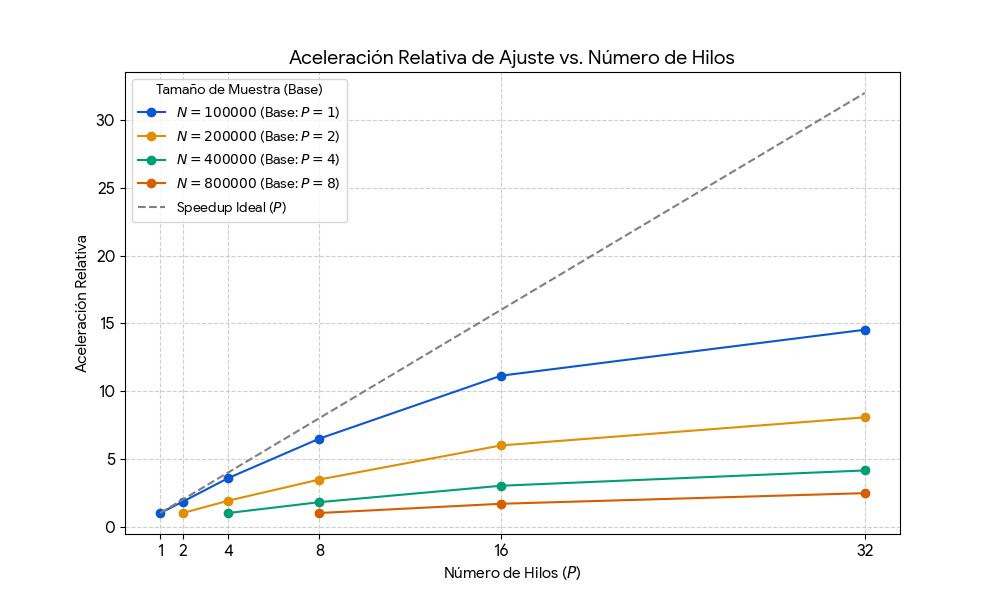
\includegraphics[width=0.8\textwidth]{speedup_vs_n_jobs.png}
    \caption{Figura 2: Aceleración Relativa ($S_{rel}(P)$) vs. Número de Hilos ($P$).}
    \label{fig:aceleracion_relativa}
\end{figure}

\paragraph{Conclusiones de la Figura 2 (Aceleración Relativa):}
\begin{enumerate}
    \item \textbf{Mejor Escalabilidad Fuerte ($N=100\,000$):} La curva azul (Base $P=1$) es la única que se acerca a la línea de Speedup Ideal, alcanzando casi $15\times$ en $P=32$. Esto confirma que, para problemas con carga de trabajo pequeña, el sistema puede gestionar el paralelismo eficientemente.
    \item \textbf{Saturación con Problemas Grandes:} Para $N=800\,000$ (Base $P=8$, curva marrón), el Speedup es el más bajo ($\approx 2.5\times$ en $P=32$). Esto significa que al pasar de 8 a 32 hilos, la ganancia de tiempo es muy pequeña. El problema ya está casi completamente saturado de paralelismo en $P=8$, y el aumento de hilos a partir de ahí solo aumenta el costo de \textbf{overhead}.
    \item \textbf{Rendimientos Decrecientes:} Ambas gráficas demuestran \textbf{rendimientos decrecientes} al aumentar $P$. Las curvas de la Figura 1 se aplanan, y las curvas de la Figura 2 se separan significativamente de la línea ideal. En la práctica, utilizar más de $P=16$ ofrece una ganancia marginal que podría no justificar el uso de tantos recursos.
\end{enumerate}

\section{Ventajas y Desventajas de las Particiones SLURM}

La elección de la partición debe priorizar los objetivos del trabajo (iteración rápida vs. ejecución final), ya que el rendimiento de cómputo por núcleo es similar.

\subsection{Partición \texttt{debug}}
\textbf{Ventajas:}
\begin{itemize}
    \item \textbf{Inicio Rápido:} Alta prioridad y baja latencia en la cola, esencial para \textbf{depuración} y \textbf{pruebas iniciales} (Validación de código).
    \item \textbf{Ciclo de Desarrollo Ágil:} Permite verificar rápidamente la configuración de recursos y la lógica del código sin largos tiempos de espera.
\end{itemize}

\textbf{Desventajas:}
\begin{itemize}
    \item \textbf{Límites Estrictos de Recursos:} Imposición de un \textbf{tiempo máximo de pared} muy limitado (ej. 30 minutos).
    \item \textbf{Inadecuada para Producción:} No permite ejecutar problemas grandes (como el caso de $N=800\,000$ con $P=32$) o tareas que requieren muchas horas de cómputo.
\end{itemize}

\subsection{Partición \texttt{standard}}
\textbf{Ventajas:}
\begin{itemize}
    \item \textbf{Producción y Larga Duración:} Diseñada para \textbf{ejecuciones finales} que requieren grandes asignaciones de tiempo y recursos.
    \item \textbf{Escalabilidad Realista:} Permite ejecutar el rango completo de problemas probados, proporcionando la base más adecuada para el \textbf{análisis de rendimiento formal} y producción.
\end{itemize}

\textbf{Desventajas:}
\begin{itemize}
    \item \textbf{Mayor Tiempo de Espera en Cola:} Los trabajos suelen tener una \textbf{menor prioridad}, lo que resulta en tiempos de espera significativos antes de la ejecución.
    \item \textbf{Ineficiente para Debugging:} Su uso es ineficiente para el desarrollo debido a la interrupción del ciclo de prueba-error por los tiempos de espera.
\end{itemize}

\end{document}